% Author: Robert Papanicola
% Source: http://www.sciences-indus-cpge.apinc.org/Schema-blocs-avec-PGF-TIKZ-sous
\documentclass{article}

\usepackage{schemabloc}

\usetikzlibrary{circuits}
\usepackage{verbatim}

\begin{comment}
:Title: Schemabloc
:Tags: Block diagrams, Macro packages

Demonstration of schemabloc_, a set of convenient macros for drawing block diagrams.
Documentation_ is only available in French, but the code examples are easy to follow.

`Download schemabloc`_

.. _download schemabloc: http://www.sciences-indus-cpge.apinc.org/IMG/zip/schema-bloc.zip
.. _documentation: http://www.sciences-indus-cpge.apinc.org/IMG/pdf/schema-bloc.pdf
.. _schemabloc: http://www.sciences-indus-cpge.apinc.org/Schema-blocs-avec-PGF-TIKZ-sous

:Author: `Robert Papanicola <http://www.sciences-indus-cpge.apinc.org/_Papanicola-Robert_>`_
:Source: `Sch�ma-blocs avec PGF/TIKZ sous LaTeX <http://www.sciences-indus-cpge.apinc.org/Schema-blocs-avec-PGF-TIKZ-sous>`_

\end{comment}

\begin{document}

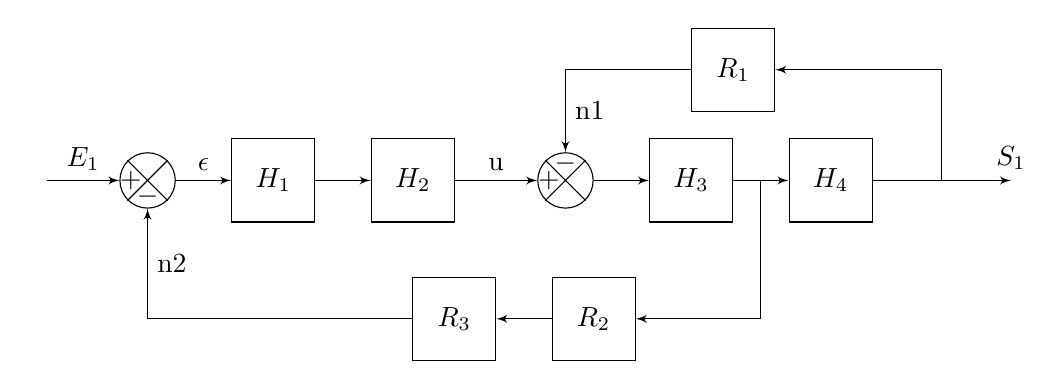
\begin{tikzpicture}
    \sbEntree{E}
    \sbComp{a}{E}
    \sbBloc{b}{$H_1$}{a}
            \sbRelier[$E_1$]{E}{a}
    \sbBlocL{c}{$H_2$}{b}
            \sbRelier[$\epsilon$]{a}{b}
    \sbComph{d}{c}
            \sbRelier[u]{c}{d}
    \sbBlocL{e}{$H_3$}{d}
    \sbBlocL{f}{$H_4$}{e}
    \sbSortie[5]{S1}{f}
            \sbRelier{f}{S1}
            \sbNomLien[0.8]{S1}{$S_1$}
    \sbDecaleNoeudy[-4]{f}{u}
    \sbDecaleNoeudy{e}{v}
    \sbBlocr{r1}{$R_1$}{u}
    \sbBlocr{r2}{$R_2$}{v}
    \sbBlocrL{r3}{$R_3$}{r2}
    \sbRelieryx{f-S1}{r1}
    \sbRelierxy[n1]{r1}{d}
    \sbRelieryx{e-f}{r2}
    \sbRelierxy[n2]{r3}{a}
\end{tikzpicture}

\end{document}
